\documentclass[12pt]{article}
\title{EE445M Lab 3}
\author{Hershal Bhave (hb6279) and Eric Crosson (esc625)}
\date{Due Sometime Soon}

\usepackage[in]{fullpage}
\usepackage{listings}
\usepackage{cleveref}
\usepackage[nosolutionfiles]{answers}
\usepackage{graphicx}
\usepackage{xcolor}
\usepackage{color}
\usepackage{enumerate}

\newenvironment{Ex}{\textbf{Problem}\vspace{.75em}\\}{}
\Newassociation{solution}{Soln}{Answers}
\pagebreak[3]
\newcommand{\Opentesthook}[2]{\Writetofile{#1}{\protect\section{#1: #2}}}
\renewcommand{\Solnlabel}[1]{\textbf{Solution}\quad}
\newcommand{\todo}{{\LARGE \emph{\color{red}TODO}}}

\newcommand{\dd}[1]{\:\mathrm{d}{#1}}
\newcommand{\ddt}[1]{\frac{\dd{}}{\dd{#1}}}
\newcommand{\dddt}[1]{\frac{\dd{}^2}{\dd{#1}^2}}

\definecolor{mygreen}{rgb}{0,0.6,0}
% \definecolor{mygreen}{rgb}{0.13,0.55,0.13}
\definecolor{mygray}{rgb}{0.5,0.5,0.5}
\definecolor{mymauve}{rgb}{0.58,0,0.82}

\lstset{
  backgroundcolor=\color{white},
  basicstyle=\scriptsize\ttfamily,
  breakatwhitespace=false,
  breaklines=true,
  captionpos=b,
  commentstyle=\color{mygreen},
  deletekeywords={...},
  escapeinside={\%*}{*)},
  extendedchars=true,
  frame=single,
  keywordstyle=\color{blue},
  % language=Octave,
  % numbers=left,
  % numbersep=5pt,
  % numberstyle=\tiny\color{mygray},
  rulecolor=\color{black},
  showspaces=false,
  showstringspaces=false,
  showtabs=false,
  % stepnumber=2,
  stringstyle=\color{mymauve},
  tabsize=2,
  title=\lstname,
  columns=fullflexible,
}

\begin{document}
\maketitle

\section{Objectives}
\begin{enumerate}
\item Extend the RTOS to include blocking and priority
\item Extend the RTOS to include two real-time periodic tasks
\item Develop minimally invasive tools to determine performance
  measures
\item Record debugging/performance data and download this data to the
  PC
\end{enumerate}

\section{Hardware Design}
No hardware design required for this lab.

\section{Software Design}
\begin{enumerate}
\item Printout of main program used to measure time jitter in
  Procedure 2

Reference \cref{lst:hardware-implementation}.
\item Printout of main program used test the blocking semaphores Preparation 4

Reference \cref{lst:test-debounce}.
\item Printout of your blocking/priority RTOS, os.c and any associated assembly files

Reference \cref{lst:test-combination,lst:os-implementation,lst:os-header}.
\end{enumerate}
\section{Measurement Data}
\begin{enumerate}
\item Plot of the logic analyzer running the
  blocking/sleeping/killing/round-robin system.

  Reference \cref{fig:round-robin}.
  \begin{figure}
    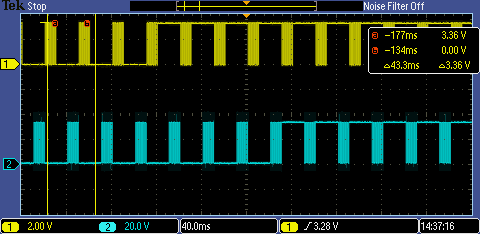
\includegraphics{img/TEK00002}
    \caption{The operating system running a purely round-robin scheduler}
    \label{fig:round-robin}
  \end{figure}

\item Plot of the scope window running the
  blocking/sleeping/killing/priority system.

  Reference \cref{fig:edf}.
  \begin{figure}
    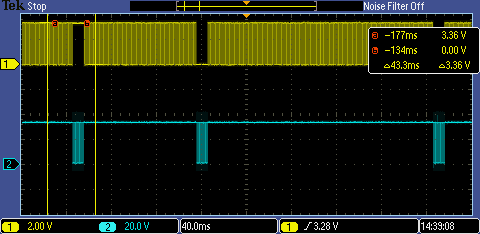
\includegraphics{img/TEK00003}
    \caption{The operating system running an EDF scheduler}
    \label{fig:edf}
  \end{figure}
\item Table like Table 3.1 each showing performance measurements
  versus sizes of the Fifo and timeslices.

\end{enumerate}
\section{Analysis and Discussion}

\begin{enumerate}[1)]
\item How would your implementation of \verb|OS_AddPeriodicThread| be
  different if there were 10 background threads? \\

  It would not be different; we designed it without 'arbitrary limits.'
\item How would your implementation of blocking semaphores be
  different if there were 100 foreground threads? \\

  It would not be different; we designed it without 'arbitrary limits.'
\item How would your implementation of the priority scheduler be
  different if there were 100 foreground threads? \\

  It would not be different; we designed it without 'arbitrary limits.'
\item What happens to your OS if all the threads are blocked? If your
  OS would crash, describe exactly what the OS does? What happens to
  your OS if all the threads are sleeping? If your OS would crash,
  describe exactly what the OS does? If you answered crash to either
  or both, explain how you might change your OS to prevent the crash. \\

  If every thread is blocked, our EDF scheduler idles until a thread
  appears in the set of Ready FIFOs. If all threads are sleeping, the
  same behavior is exhibited.
\item What happens to your OS if one of the foreground threads
  returns? E.g., what if you added this foreground
  % TODO: format
  \begin{verbatim}
    void BadThread(void){
      for(int i=0; i<100; ++i) {};
    }
  \end{verbatim}
  What should your OS have done in this case? Do not implement it,
  rather, with one sentence, say what the OS should have done? \\

  Our OS would crash due to stack underflow, but the OS could use
  different stacks for OS and user code (MSP and PSP) so that a
  recovery is possible.
\item What are the advantages of spinlock semaphores over blocking
  semaphores? What are the advantages of blocking semaphores over
  spinlock? \\

  Blocking semaphores allow other threads to run; spinlock semaphores
  are easier to program.
\item Consider the case where thread T1 interrupts thread T2, and we
  are experimentally verifying the system operates without critical
  sections. Let n be the number of times T1 interrupts T2. Let m be
  the total number of interruptible locations within T2. Assume the
  time during which T1 triggers is random with respect to the place
  (between which two instructions of T2) it gets interrupted. In other
  words, there are $m$ equally-likely places within T2 for the T1
  interrupt to occur. What is the probability after n interrupts that
  a particular place in T2 was never selected? Furthermore, what is
  the probability that all locations were interrupted at least once?
\end{enumerate}

\section{Code}
\lstinputlisting[language=C,label=lst:os-implementation,caption=\texttt{os.c}]{@doc-staging-area@/os.c}
\lstinputlisting[language=C,label=lst:os-header,caption=\texttt{os.h}]{@doc-staging-area@/os.h}
\lstinputlisting[language=C,label=lst:hardware-implementation,caption=\texttt{hardware.c}]{@doc-staging-area@/hardware.c}
\lstinputlisting[language=C,label=lst:test-combination,caption=\texttt{test-combination.c}]{@doc-staging-area@/test-combination.c}
\lstinputlisting[language=C,label=lst:test-debounce,caption=\texttt{test-debounce.c}]{@doc-staging-area@/test-debounce.c}

\end{document}
